\documentclass[11pt,a4paper,twoside,openright]{book}
%\documentclass[a4paper,12pt,fourier,numbered,print,index]

% CHECK https://www.writelatex.com/1283488jybyzp#/3132576/
%%------------------------ PACKAGES------------------------------
%%------------------------ BOOLEANS FOR OPTIONS -------------------------------
\usepackage{ifthen}

\newboolean{enable_backrefs} % enable backrefs in the bibliography
\newboolean{enable_line_numbers}
\newboolean{enable_visual_comments}
\newboolean{enable_animations}
%%------------------------ Personal Commands -------------------------------

\newcommand{\myTitle}{Modeling and Simulation of Macrosegregation Induced by Thermomechanical Deformation in Steels\xspace}
%\newcommand{\mySubtitle}{\textsf{New} technique to solve \textsf{Old} problems !\xspace}
\newcommand{\myDegree}{Ph.D.\xspace}
\newcommand{\myName}{Ali SAAD\xspace}
\newcommand{\profMB}{Michel BELLET\xspace}
\newcommand{\profCAG}{Charles-Andre GANDIN\xspace}
\newcommand{\myFaculty}{MINES ParisTech\xspace}
\newcommand{\myDepartment}{Material Forming Center\xspace}
\newcommand{\myUni}{PSL Research University\xspace}
\newcommand{\myLocation}{France\xspace}
\newcommand{\myTime}{December 2014\xspace}
\newcommand{\myVersion}{version 1.0\xspace}

%\newcommand{\profCEMEFone}{Michel BELLET\xspace}
%\newcommand{\profCEMEFtwo}{Charles-Andre GANDIN\xspace}
%\newcommand{\profTSVone}{Olivier JAOUEN\xspace}
%\newcommand{\profTSVtwo}{Frederic COSTES\xspace}
%\newcommand{\profTSVthree}{Guillaume FRANCOIS\xspace}

%%------------------------ Classic Thesis Commands -------------------------------
%% Define \cleardoublepgage
\makeatletter
\def\cleardoublepage{\clearpage\if@twoside \ifodd\c@page\else
    \hbox{}
    \thispagestyle{empty}
    \newpage
    \if@twocolumn\hbox{}\newpage\fi\fi\fi}
\makeatother \clearpage{\pagestyle{plain}\cleardoublepage}

%%------------------------ FONTS -------------------------------
%\usepackage{lmodern}
%\usepackage{fouriernc}
\usepackage{fourier} 		% Utopia font-typesetting including mathematical formula compatible with newer TeX-Distributions (>2010)
%\usepackage{utopia} 		% on older systems -> use this package instead of fourier in combination with mathdesign for better looking results
%\usepackage[adobe-utopia]{mathdesign}
%\usepackage{ae,aecompl}

%------------------------ LANGUAGES-FRENCH ACCENTS -------------------------------
\usepackage[utf8]{inputenc}
% For the front page
\usepackage[T1]{fontenc}		
\usepackage[francais, english]{babel} % american
%\usepackage{utopia} % lmodern % utopia % fourier

%%------------------------ ACRONYMS -------------------------------
%\usepackage[printonlyused,smaller]{acronym}
%\renewcommand{\bflabel}[1]{{#1}\hfill} % fix the list of acronyms

%%------------------------ BIBLIOGRAPHY NATBIB (deprecated) -------------------------------
% http://merkel.zoneo.net/Latex/natbib.php
% default option for citation rendering is "authoryear" and "round" brackets
% sort: orders multiple citations into the sequence in which they appear in the list of references;
% sort&compress: as sort but in addition multiple numerical citations are compressed if possible (as 3-6, 15);

%\usepackage[square,numbers]{natbib}    % number in square , useful to add sortcompress
%\usepackage[square,sort]{natbib} % name and year in square

%%------------------------ BIBLIOGRAPHY BIBLATEX -------------------------------
\usepackage{csquotes}% Recommended
\usepackage [backend=bibtex,style=authoryear]{biblatex} %style=authoryear %style=apa

% Rename citation commands (instead of redefining them, impossible then to use optional "see" or page number
\let\citep\parencite
\let\citet\textcite
% (deprecated)
%\newcommand{\citep}[1]{\parencite{#1}}
%\newcommand{\citet}[1]{\textcite{#1}}

\ExecuteBibliographyOptions{hyperref=true,
							backref=true,
							firstinits=true, 
							isbn=false, 
							eprint=false,
							url=true, 
							doi=false, 
							sorting=nyt, 
							minnames=1, 
							maxcitenames=1, % in text citations, allows suffix a,b ...
							maxbibnames=5,
							alldates=short, 
							punctfont=true, 
							autopunct=false, 
							block=none, 
							dashed=false}
% bibresource moved to "main.tex" to allow autcomplete in TexMaker
%\addbibresource{References/auto_references.bib}

% Spacing
\setlength{\bibitemsep}{10pt} %vertical spacing
\setlength{\bibhang}{1cm} %label alignment (0 for perfect align)

% Disable URL dates
\AtEveryBibitem{%
    \clearfield{urldate}%
    \clearfield{urlday}%
    \clearfield{urlmonth}%
    \clearfield{urlyear}%
    \clearlist{language}
}%

%Fix the comma problem after the journal name (via addcomma)
\DeclareFieldFormat{journaltitle}{\mkbibemph{#1\isdot}\addcomma\space}

%Fix number and volume format
\renewbibmacro*{volume+number+eid}{%
  \printfield{volume}%
%  \setunit*{\adddot}% DELETED
  \setunit*{\addnbspace}% NEW (optional); there's also \addnbthinspace
  \printfield{number}%
  \setunit{\addcomma\space}%
  \printfield{eid}}
\DeclareFieldFormat[article]{number}{\mkbibparens{#1}}

%Disable prefix "In"
\renewbibmacro{in:}{}

% Define brackets instead of parenthesis
\makeatletter
\newrobustcmd*{\parentexttrack}[1]{%
  \begingroup
  \blx@blxinit
  \blx@setsfcodes
  \blx@bibopenparen#1\blx@bibcloseparen
  \endgroup}
\AtEveryCite{%
  \let\parentext=\parentexttrack%
  \let\bibopenparen=\bibopenbracket%
  \let\bibcloseparen=\bibclosebracket}
\makeatother

%define label before reference in list	
\renewbibmacro{begentry}{%
\textbf{[\printnames[][-\value{liststop}]{labelname}~\printfield{labelyear}\printfield{extrayear}}]\\}

%define full hyperlink for textcite and parencite
% http://tex.stackexchange.com/questions/15951/hyperlink-name-with-biblatex-authoryear-biblatex-1-4b
\DeclareFieldFormat{citehyperref}{%
\DeclareFieldAlias{bibhyperref}{noformat}% Avoid nested links
\bibhyperref{#1}}
\DeclareFieldFormat{textcitehyperref}{%
\DeclareFieldAlias{bibhyperref}{noformat}% Avoid nested links
\bibhyperref{%
#1%
\ifbool{cbx:parens}
  {\bibcloseparen\global\boolfalse{cbx:parens}}
  {}}}
\savebibmacro{cite}
\savebibmacro{textcite}

\renewbibmacro*{cite}{%
\printtext[citehyperref]{%
\restorebibmacro{cite}%
\usebibmacro{cite}}}

\renewbibmacro*{textcite}{%
\ifboolexpr{
( not test {\iffieldundef{prenote}} and
  test {\ifnumequal{\value{citecount}}{1}} )
or
( not test {\iffieldundef{postnote}} and
  test {\ifnumequal{\value{citecount}}{\value{citetotal}}} )
}
{\DeclareFieldAlias{textcitehyperref}{noformat}}
{}%
\printtext[textcitehyperref]{%
\restorebibmacro{textcite}%
\usebibmacro{textcite}}}

%%------------------------ LAYOUT -------------------------------

% Package geometry is loaded ONLY to achieve a specific size in title page (SHOULD BE LOADED BEFORE CUSTOM LAYOUT SETTINGS)
\usepackage[top=1cm, bottom=1cm, left=1cm, right=1cm, headheight=15pt]{geometry}

%% --- Margins (Custom layout)
\setlength{\textwidth}{146.8mm} % = 210mm - 37mm - 26.2mm
\setlength{\oddsidemargin}{11.6mm} % 37mm - 1in (from hoffset)
\setlength{\evensidemargin}{0.8mm} % = 26.2mm - 1in (from hoffset)
\setlength{\topmargin}{-2.2mm} % = 0mm -1in + 23.2mm 
\setlength{\textheight}{221.9mm} % = 297mm -29.5mm -31.6mm - 14mm (12 to accomodate footline with pagenumber)
\setlength{\headheight}{14pt}
%% --- Paragraph spacing
\setlength{\parindent}{0pt}
%% --- Interline spacing
\usepackage{setspace} % increase interline spacing slightly
\setstretch{1.1}

%%------------------------ Captions  -------------------------------

% Captions: This makes captions of figures use a boldfaced small font. 
\RequirePackage[small,bf]{caption}
\RequirePackage[labelsep=endash,tableposition=top]{caption}  % labelsep=endash % space
\addto\captionsenglish{\renewcommand{\figurename}{Fig.}}

%%-----------------------  Footnote Header formatting -------------------------------
% From EPFL template
%\usepackage[perpage]{footmisc} %Range of footnote options 

\usepackage{fancyhdr}
\renewcommand{\sectionmark}[1]{\markright{#1}}  %\markright{\thesection\ #1}
\pagestyle{fancy}
	\fancyhf{}
	\renewcommand{\headrulewidth}{0.4pt}
	\renewcommand{\footrulewidth}{0pt}
	\fancyhead[OR]{\bfseries \nouppercase{\rightmark}}
	\fancyhead[EL]{\bfseries \nouppercase{\leftmark}}
	\fancyfoot[EL,OR]{\thepage}
\fancypagestyle{plain}{
	\fancyhf{}
	\renewcommand{\headrulewidth}{0pt}
	\renewcommand{\footrulewidth}{0pt}
	\fancyfoot[EL,OR]{\thepage}}
\fancypagestyle{addpagenumbersforpdfimports}{
	\fancyhead{}
	\renewcommand{\headrulewidth}{0pt}
	\fancyfoot{}
	\fancyfoot[RO,LE]{\thepage}
}

%%------------------------ Figures  -------------------------------
%\usepackage{rotating}
%\usepackage{wrapfig}
%\usepackage{float}
%\usepackage{subfig} %note: subfig must be included after the `caption` package.
\usepackage{subcaption}
 

% \usepackage{graphicx,xcolor}
\usepackage[dvipsnames]{xcolor}
\definecolor{webgreen}{rgb}{0,.5,0}
\definecolor{webbrown}{rgb}{.6,0,0}
\definecolor{Maroon}{cmyk}{0, 0.87, 0.68, 0.32}
\definecolor{RoyalBlue}{cmyk}{1, 0.50, 0, 0}

%\graphicspath{{images/}}
\makeatletter
\setlength{\@fptop}{0pt}  % for aligning all floating figures/tables etc... to the top margin
\makeatother

%%------------------------ Tables  -------------------------------
%\usepackage{longtable}
%\usepackage{multicol}
%\usepackage{multirow}
%\usepackage{tabularx}

%\usepackage{booktabs}

%%------------------------ Math and SI Units  -------------------------------
\usepackage{amsfonts}
\usepackage{amsmath}
\usepackage{amssymb}
\usepackage[mathscr]{euscript}
\usepackage{siunitx} % http://ftp.oleane.net/pub/CTAN/macros/latex/contrib/siunitx/siunitx.pdf
% \num{.3e45}   ,  \num{3.45d-4}   , \numlist{10;30;50;70} ,  \numrange{10}{30} , 

%%------------------------ Cross References  -------------------------------
% --- Hyperref and Options
\usepackage{hyperref}
\hypersetup{%
	% --------------
	% PDF Display
	% --------------
    linktocpage=false, % make page number, not text, be link on TOC, LOF and LOT
    linktoc=all,
    pdfstartpage=1, 
    pdfstartview=FitV, % FitR (rectangle) % FitH %FitV % FitB (bounding box) % FitBH % FitBV
    %
    breaklinks=true, 
    pageanchor=true,  % put an anchor on every page, DO NOT TURN OFF
    pdfpagemode=UseOutlines,  % UseNone % UseOutlines (shows bookmarks) % UseThumbs
    plainpages=false, % Forces page anchors to be named by the Arabic form of the page number, rather than the formatted form.
	%
    bookmarksnumbered, 
    bookmarksopen=false, 
    bookmarksopenlevel=3,%
	pdfpagelayout=TwoPageRight,  % SinglePage % TwoPageLeft % TwoPageRight
	hypertexnames=true, % use guessable names for links, DO NOT TURN OFF
    pdfhighlight=/O, % How link buttons behave when selected; /I is for inverse (the default) /N (no effect), /O (outline), and /P (inset highlighting).
	%
	% --------------
	% Hyperlink Colors
	% --------------  
	colorlinks=true,  
    urlcolor=webbrown, %webbrown %Black
    linkcolor=RoyalBlue, %RoyalBlue, %Black
    citecolor=webgreen, %webgreen, %Black
    pagecolor=RoyalBlue,%Black
	% --------------
    % PDF Information
	% --------------  
    pdftitle={\myTitle},%
    pdfauthor={\myName, \myUni, \myFaculty},%
    pdfkeywords={Macrosegregation, solidification, level set, numerical simulation}%
}


%% --- cleveref (should always be invoked AFTER hyperref)
%\usepackage{cleveref}
\usepackage[nameinlink]{cleveref} % capitalize


\DefineBibliographyStrings{english}{%
  backrefpage = {cited on page},% originally "cited on page"
  backrefpages = {cited on pages},% originally "cited on pages"
}

%% --- beckref and Options (NATBIB compatible - Obsolete)
%\newcommand{\backrefnotcitedstring}{\relax}%(Not cited.)
%\newcommand{\backrefcitedsinglestring}[1]{(cited on page~#1)}
%\newcommand{\backrefcitedmultistring}[1]{(cited on pages~#1)}
%\ifthenelse{\boolean{enable_backrefs}}%
%{%
%		\usepackage[hyperpageref]{backref}  % to be loaded after hyperref package
%		   \renewcommand{\backreftwosep}{ and~} % separate 2 pages
%		   \renewcommand{\backreflastsep}{, and~} % separate last of longer list
%		   \renewcommand*{\backref}[1]{}  % disable standard
%		   \renewcommand*{\backrefalt}[4]{% detailed backref
%		      \ifcase #1 %
%		         \backrefnotcitedstring%
%		      \or%
%		         \backrefcitedsinglestring{#2}%
%		      \else%
%		         \backrefcitedmultistring{#2}%
%		      \fi}%
%}%{\relax}    

%%--------------------- TOC --------
%\setcounter{secnumdepth}{2}
%\setcounter{tocdepth}{2}

\usepackage{minitoc} % use like this : \minitoc 
\setcounter{minitocdepth}{2}
\setlength{\mtcindent}{24pt} 
\renewcommand{\mtcfont}{\small\rm}
\renewcommand{\mtcSfont}{\small\bf}


%%------------------------ NOMENCLATURE / GLOSSARY -------------------------------
% http://www.latex-community.org/know-how/latex/55-latex-general/263-glossaries-nomenclature-lists-of-symbols-and-acronyms
%\usepackage[toc]{glossaries}
% use it like: \newglossaryentry{label}{definition}
%\usepackage[xindy,toc]{glossaries}  
%\makeglossaries 


%%------------------------ Names of sections for figures, nomenclature ...  -------------------------------
% To change the name of the Nomenclature section, uncomment the following line
%\renewcommand{\contentsname}{My Table of Contents}
%\renewcommand{\listfigurename}{My List of Figures}
%\renewcommand{\listtablename}{My List of Tables}
%\renewcommand{\nomname}{Symbols}

%%------------------------ Appendix -------------------------------
\usepackage[titletoc]{appendix}
% The default value of both \appendixtocname and \appendixpagename is `Appendices'. These names can all be changed via: 
%\renewcommand{\appendixtocname}{List of appendices}
\renewcommand{\appendixname}{Appendicitis}

%%------------------------ MISC PACKAGES -------------------------------
% Graphs
\usepackage{pgfplots}
\pgfplotsset{width=8cm,compat=newest}
%\usepgfplotslibrary{external}
%\tikzexternalize

% Format URLs
\usepackage{url}

% Input dummy text
\usepackage{lipsum}

\usepackage{pdfpages} %\includepdf[options]{filename}
%\usepackage{algpseudocode} 

% Display line number
\usepackage{lineno}
\ifthenelse{\boolean{enable_line_numbers}}%
{%
	%\linenumbers
	\pagewiselinenumbers % requires compiling AT LEAST twice
}{\relax}    

% Comments
\usepackage{todonotes}
\ifthenelse{\boolean{enable_visual_comments}}%
{% then
   \newcommand{\comment}[2][]{\todo[backgroundcolor=yellow!50!white, caption={#2}, inline, size=\small, #1]{\renewcommand{\baselinestretch}{0.5}\selectfont#2\par}}
}
{% else 
  \newcommand{\comment}[2][]{}
}

% Enchance syllable breaking avoiding bad boxes
\usepackage[stretch=10]{microtype} % which allows font expansion up to 1% (default is 2%)

% Cancel sign in math equations
\usepackage{cancel}

% Enables putting the pdf_tex graphics in a subfolder
\usepackage{import}

% Frontpage packages (Dorian)
\usepackage{eso-pic}	% Nécessaire pour mettre des images en arrière plan
%\usepackage[top=1cm, bottom=1cm, left=1cm, right=1cm, headheight=15pt]{geometry}
%\usepackage{graphicx}
%\usepackage{array}		% Permet d'écrite 'THESE' de haut en bas


%%------------------------ ENVIRONMENTS  -------------------------------
% Change hyperlink color to black in miniTOC, TOC, TOF ...
\newenvironment{nolinkcolors}[1]{\begingroup \hypersetup{hidelinks}  #1 }{\endgroup}

%% Dorian Depriester: Figures centrées, et en position 'here, top, bottom or page'
\newenvironment{figureth}[3]{
		\begin{figure}[htbp]
			\centering
			\includegraphics[width=#1\textwidth]{#2}
			\caption{#3}
			%\label{fig:#4}
	}{
		\end{figure}
		}

% USE LIKE THIS	
%\begin{figureth}
% textwidth 
%{•}
%path 
%{•}
% caption
%{•}
% label
%{•}
%\end{figureth}

\newenvironment{figurethmulti}{
		\begin{figure}[htbp]
			\centering
	}{
		\end{figure}
		}

%**********
%% Tableaux centrés, et en position 'here, top, bottom or page'
\newenvironment{tableth}{
		\begin{table}[htbp]
			\centering
			
	}{
		\end{table}
		}
%**********	
\newenvironment{subfigureth}[2]{
		\begin{subfigure}[t]
			\centering
			\includegraphics[width=#1\textwidth]{#2}
			%\caption{#3}
			%\label{fig:#4}
	}{
		\end{subfigure}
		}
%**********	


%%------------------------ BEGIN  -------------------------------
\begin{document}

\lipsum[4-57]

\frontmatter
\begin{titlepage}
%\maketitle
\end{titlepage}

%\include{Dedication/dedication}
%\include{Declaration/declaration}
%\cleardoublepage
\section*{Acknowledgement}
%\addcontentsline{toc}{section}{Acknowledgement}

I would like to thank the CEMEF laboratory, giving me the opportunity to study in the prestigious MINES ParisTech.
\newline
\newline
I would like to thank my directors, Dr. Charles-André Gandin and Pr. Michel Bellet, for their
guidance, support, and inspiration through my Ph.D. years.
I am grateful to Pr. Hervé Combeau and Pr. Markus Rettenmayr for the thesis report 
and the valuable expertise they brought to my work. I am also sincerely grateful to Pr. Florian Kargl for the examination of this dissertation.
This work has been supported by the European Space Agency. Its financial support for the research project CCEMLCC-2 is also gratefully acknowledged.
\newline
\newline
I would like to thank the members of our research group, especially Dr. Charles-André for all the technical discussions. 
I am also grateful to Dr. Tommy Carozzani for the valuable advices on my work and for the professional inspiration.
I thank also all the colleagues who influenced me in a way or in another: Jose, Shijia, Thi-Thuy-Mi, Alexis, Dorian, Sabrina, Xavier, Dr. Michel K, Hitti Drs and Masri Drs ... (and the list goes on).\newline
I am very thankful to Dr. Elie Hachem for the moral and scientific push in the last few miles before the thesis defence.
I am indebted to Dr. Frédéric Costes for continuously believing in my work and for giving me the opportunity
to continue my career in computational material science at TRANSVALOR.
\newline
\newline
I thank Rabih for being a great source of inspiration and discipline. The accomplishment of this work wouldn't have been possible without the unconditional support and love of the most important women in my life: my wife and my mother. 
\newline
\newline
Isn't life complex, complicated and beautiful at the same time ?
%\include{Abstract/abstract}

% *********************** Adding TOC and List of Figures ***********************
\tableofcontents

\listoffigures
\lipsum[20]
\listoftables 
\lipsum[20]
% \printnomenclature[space] space can be set as 2.5cm between symbol and
% description
%\printnomencl

%%------------------------ MAIN MATTER  -------------------------------

\mainmatter

\chapter{Modelling Review}
\minitoc
\newpage

In this chapter the following points are discussed
\begin{itemize}
\item what does a typical solidifications problem consist of ? heat - fluid - solid 
- chemical species
\item what are the modeling scales of these physics ? direct (micro: phase field / macro: CA) 
and indirect (micro Nancy models / macro: current FE model)
\comment{Maybe worth showing the 2x2 table that CAG showed at the ICASP conference ?}
\item Overview of these models ??
\item Presence of AIR requires a new problem definition : Lagrangian or Eulerian framework
\end{itemize}


\section{FE model}
A section presenting the main FE equations that will be solved in the metal being a single domain.
\begin{itemize}
\item Energy (chapter 1)
\item
\end{itemize}

\comment{talking about Eulerian approach Air Metal will be presented in the next chapters}

\section{Biblio test}
\cite{carozzani_direct_2013} are going to appear in the paper 
%\include{Chapter7/chapter7}

%%------------------------ BACK MATTER  -------------------------------

% Backmatter should be commented out, if you are using appendices after References
%\backmatter 

% ********************************** Bibliography ******************************
%\begin{spacing}{0.9}

% To use the conventional natbib style referencing
% Bibliography style previews: http://nodonn.tipido.net/bibstyle.php

%\bibliographystyle{apalike}
%\bibliographystyle{plainnat} % use this to have URLs listed in References
%\cleardoublepage
%\bibliography{References/references} % Path to your References.bib file


% If you would like to use BibLaTeX for your references, pass `custombib' as 
% an option in the document class. The location of 'reference.bib' should be 
% specified in the preamble.tex file in the custombib section. 
% Comment out the lines related to natbib above and uncomment the following line.

% \printbibliography[heading=bibintoc, title={References}]

%end{spacing}

% ********************************** Appendices ********************************

%\begin{appendices} % Using appendices environment for more functunality

%\chapter{Notes}

from \url{http://aerojet.engr.ucdavis.edu/fluenthelp/html/ug/node572.htm} \\

For many natural-convection flows, you can get faster convergence with the Boussinesq model than 
you can get by setting up the problem with fluid density as a function of temperature. This model 
treats density as a constant value in all solved equations, except for the buoyancy term in the momentum 
equation:
\begin{align}
 (\rho - \rho_0) g \approx -\rho_0 \beta (T - T_0) g 	
\end{align}

where  $\rho_0$ is the (constant) density of the flow,  $T_0$ is the operating temperature, and  $\beta$ is 
the thermal expansion coefficient. Equation  13.2-18 is obtained by using the Boussinesq approximation  
$\rho = \rho_0 (1 - \beta \Delta T)$ to eliminate  $\rho$ from the buoyancy term. This approximation is accurate as 
long as changes in actual density are small; specifically, the Boussinesq approximation is valid when  $\beta(T-T_0)\ll 1$.
%\chapter{Boundary conditon analysis in non level set simulations}

\comment{this appendix is temporary, it may be deleted later}

We want to understand the consequence of removing the no-slip boundary condition at the \emph{M-A} boundary and compare the effect on macrosegregation. 
For computations without level set, as previously done in chapter 4 for the \emph{Tsolver}'s validation in convection-diffusion regimes, 
a no-slip condition was applied for all domain boundaries.
However, this is not readily implemented with the level set method which considers the local interface velocity for its transport.
In \cref{fig:slipbc_2800,fig:slipbc_7000}, we compare at 2800 s and 7000 s the differences between a no-slip condition on the top boundary 
and a free-slip tangential condition, assuming zero normal velocity. 

%-----------------
\begin{figure}[htbp]
\centering
   %------------
  \begin{subfigure}[t]{0.4\textwidth}
    \centering
  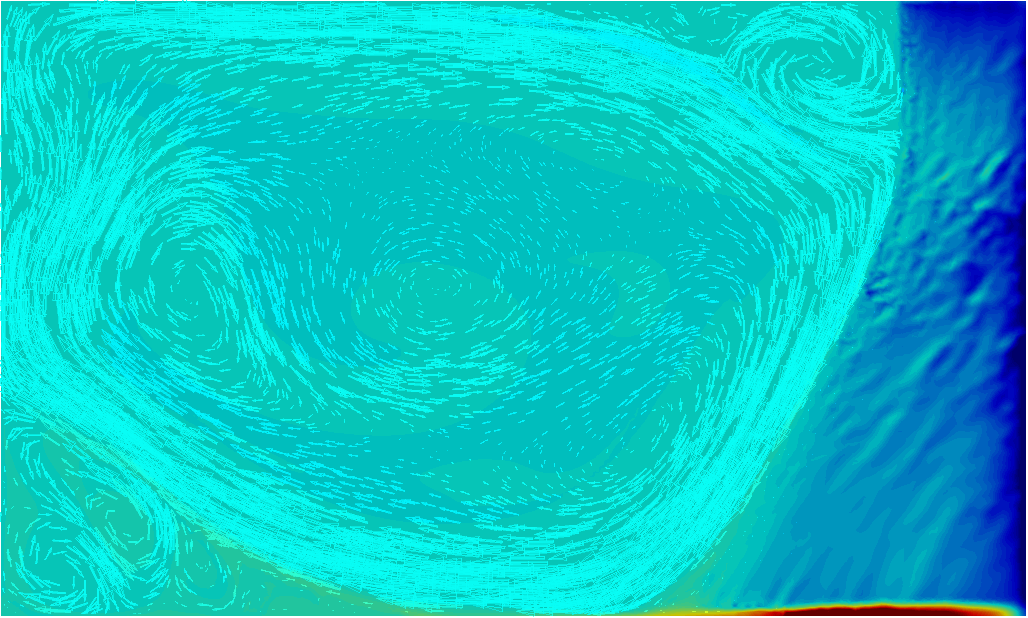
\includegraphics[width=\textwidth]{Chapter5/Graphics/2d/ref_2800s_nosliptop.png}
  \caption{}
    \label{fig:noslip2800}
  \end{subfigure}
  %------------------------------
  \begin{subfigure}[t]{0.15\textwidth}
    \centering
  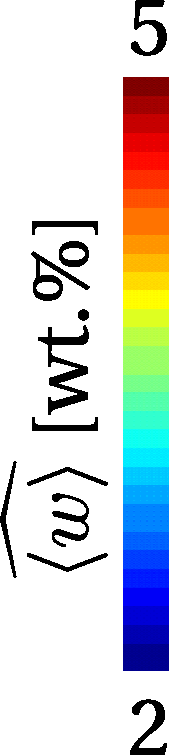
\includegraphics[width=0.3\textwidth]{Chapter5/Graphics/2d/colorbar_w.pdf}
  \end{subfigure}
  %------------------------------
  \begin{subfigure}[t]{0.4\textwidth}
    \centering
  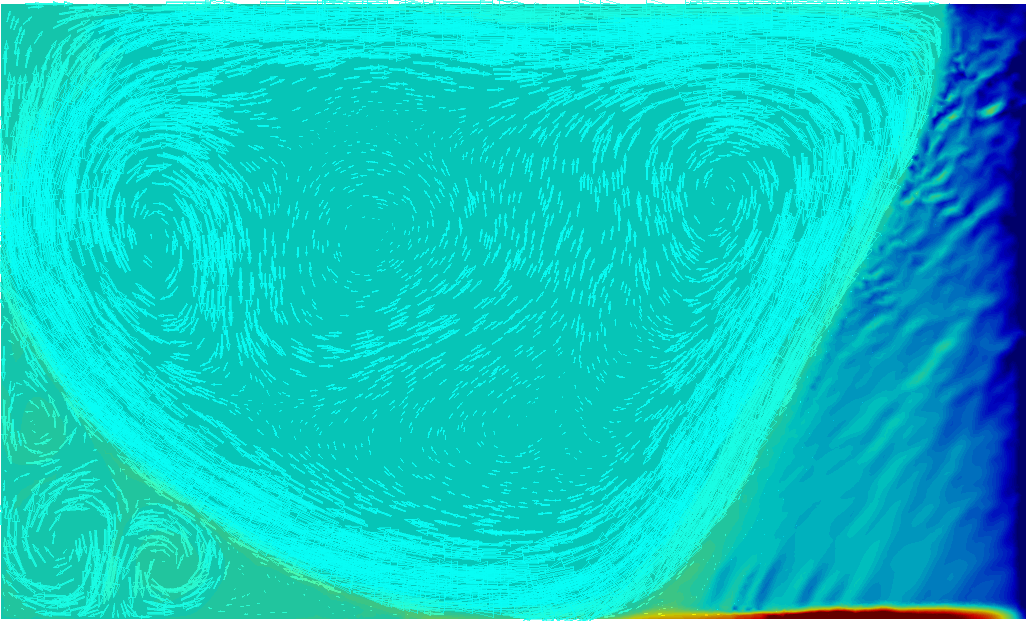
\includegraphics[width=\textwidth]{Chapter5/Graphics/2d/ref_2800s_sliptop.png}
  \caption{}
    \label{fig:freeslip2800}
  \end{subfigure}
   %------------
\caption{Comparison of two solidification with macrosegregation cases assuming (a) a no-slip condition on the upper boundary 
or (b) a tangential free-slip condition. The snapshots are taken at 2800 s.}
\label{fig:slipbc_2800}
\end{figure}
%------------------

%-----------------
\begin{figure}[htbp]
\centering
   %------------
  \begin{subfigure}[t]{0.4\textwidth}
    \centering
  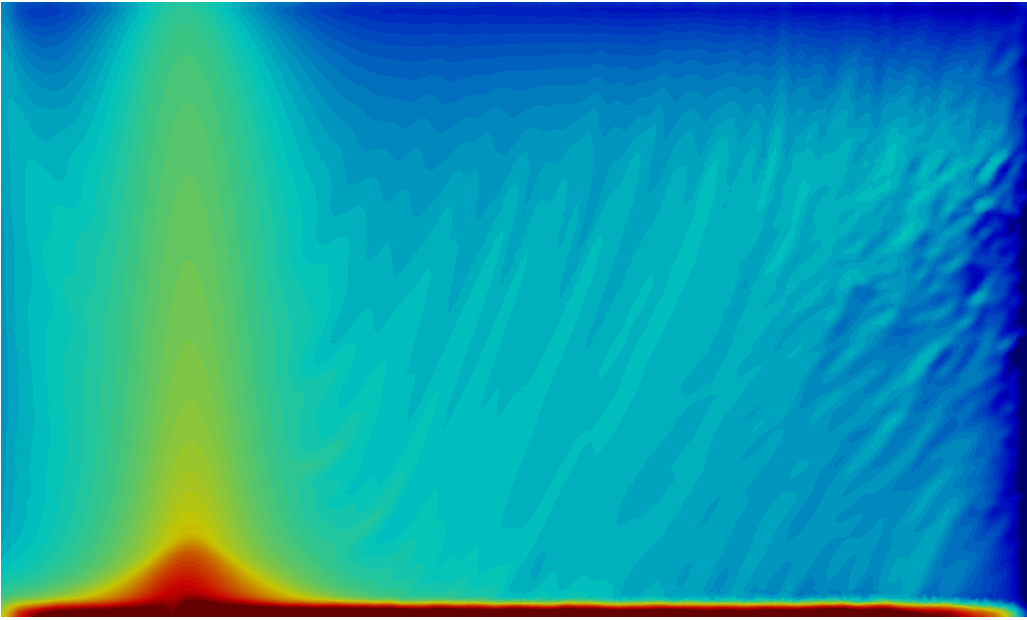
\includegraphics[width=\textwidth]{Chapter5/Graphics/2d/ref_7000s_nosliptop.png}
  \caption{}
    \label{fig:noslip7000}
  \end{subfigure}
  %------------------------------
  \begin{subfigure}[t]{0.15\textwidth}
    \centering
  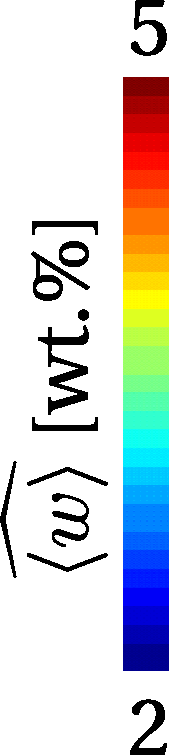
\includegraphics[width=0.3\textwidth]{Chapter5/Graphics/2d/colorbar_w.pdf}
  \end{subfigure}
  %------------------------------
  \begin{subfigure}[t]{0.4\textwidth}
    \centering
  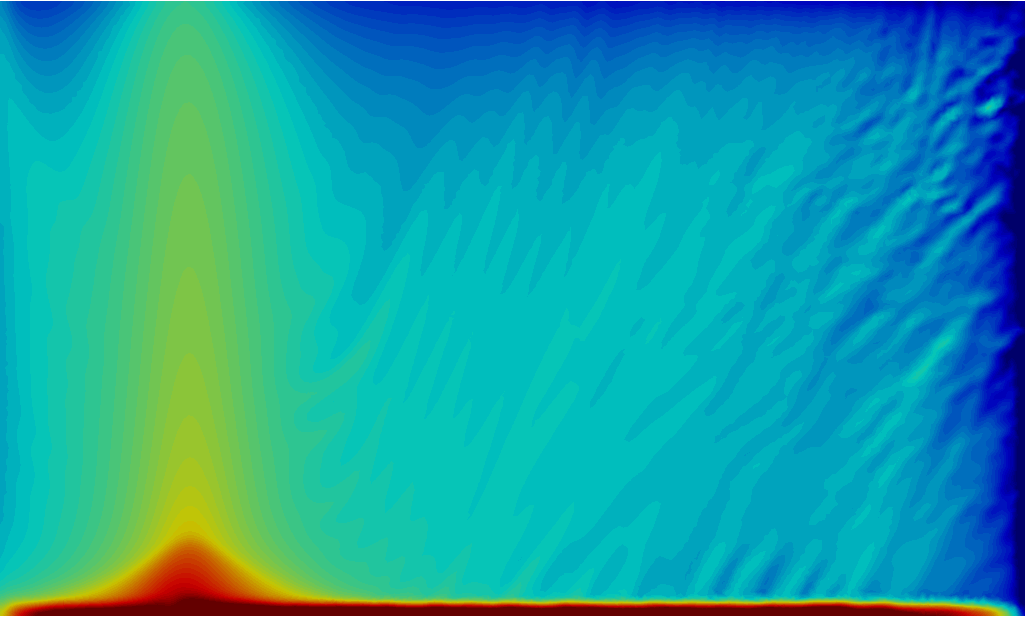
\includegraphics[width=\textwidth]{Chapter5/Graphics/2d/ref_7000s_sliptop.png}
  \caption{}
    \label{fig:freeslip7000}
  \end{subfigure}
   %------------
\caption{Comparison of two solidification with macrosegregation cases assuming (a) a no-slip condition on the upper boundary 
or (b) a tangential free-slip condition. The snapshots are taken at 7000 s.}
\label{fig:slipbc_7000}
\end{figure}
%------------------

In \cref{fig:slipbc_2800}, solidification is still at an early stage, at 2800 s. The main difference between \cref{fig:noslip2800} and 
\cref{fig:freeslip2800} is the flow pattern near the top interface. The no-slip wall acts a brake for the vicinity flow, 
deviating it downwards and allow a quicker solidification rate for the right upper part of the metal. The flow near the slip wall
in \cref{fig:freeslip2800} is not damped and therefore delays solidification of the upper corner where it impinges.
The different flow pattern creates a more pronounced negative segregation in the upper right corner of \cref{fig:noslip2800}, compared
to the same location in  \cref{fig:freeslip2800}. Later when solidification is complete at 7000 s (\cref{fig:slipbc_7000}), the overall
macrosegregation is more visible: expect for the previously mentioned difference in the corner segregation, no big differences are observed.
This means that when using the level set method, allowing the velocity to have non-zero values near the interface should not drastically  change the
predicted flow pattern and the subsequent macrosegregation.
% \section{Useful Expressions}
% \comment{ address a problem: attend to, apply oneself to, tackle, see to, deal with, confront, come to grips with, get down to, turn one's hand to, take in hand, undertake, concentrate on, focus on, devote oneself to
% "the selectmen failed to address the issue of subsidies" }
% \begin{itemize}
% \item  the basic premise = the basic argument is that ...
% \item A complication inherent in this approach is that
% \item an important objective of the present study is to
% \end{itemize}


%\end{appendices}

% *************************************** Index ********************************
%\printthesisindex % If index is present

\end{document}